% ----- formatovani dokumentu -----------------------------------------------
\documentclass[12pt,a4paper,titlepage,final]{report}
\usepackage[utf8]{inputenc}
\usepackage[T1, IL2]{fontenc}
\usepackage{graphicx}
\usepackage{epstopdf}
\usepackage[margin=2cm]{caption}
\usepackage[top=3cm, left=2cm, right=2cm, text={17cm, 24cm}, ignorefoot]{geometry}
\usepackage{color}
\usepackage{url}
\usepackage{setspace}
\singlespacing
\usepackage[square, numbers]{natbib}
\pagestyle{plain}
\pagenumbering{arabic}
\setcounter{page}{1}
\setcounter{secnumdepth}{-1}
\setlength{\parindent}{1cm}
\usepackage{natbib}

% ----- vyberte jazyk -------------------------------------------------------
\usepackage[english,czech]{babel}
%\usepackage[english]{babel}

% ----- dopiste titulky -----------------------------------------------------
\newcommand\Course{Pokročilá počítačová grafika}
\newcommand\WorkTitle{Distribuovaný ray tracing}
\newcommand\Author{Miloslav Číž}
\newcommand\AuthorEmail{xcizmi00@stud.fit.vutbr.cz}
\newcommand\Faculty{Fakulta Informačních Technologií}
\newcommand\School{Vysoké Učení Technické v Brně}

\usepackage[
pdftitle={\WorkTitle},
pdfauthor={\Author},
bookmarks=true,
colorlinks=true,
breaklinks=true,
urlcolor=blue,
citecolor=blue,
linkcolor=blue,
unicode=true,
]
{hyperref}


% ----- titulni strana ------------------------------------------------------

\begin{document}
    \begin{titlepage}
    \begin{center}
        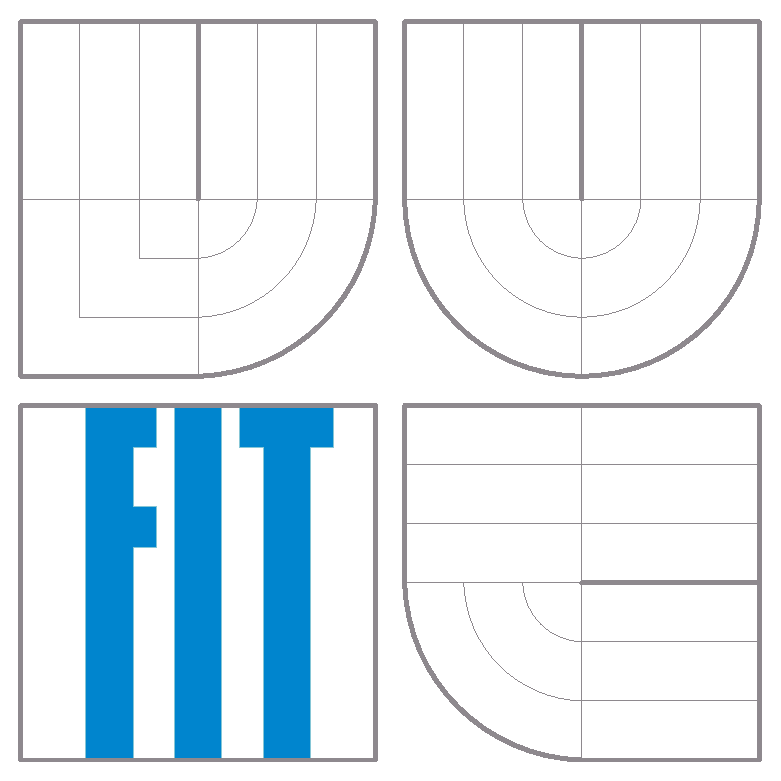
\includegraphics[height=5cm]{images/logo.eps}
    \end{center}
    \vfill
    \begin{center}
        \begin{Large}
            \Course\\
        \end{Large}
        \bigskip
        \begin{Huge}
            \WorkTitle\\
        \end{Huge}
    \end{center}
    \vfill
    \begin{center}
        \begin{large}
            \today
        \end{large}
    \end{center}
    \vfill
    \begin{flushleft}
        \begin{large}
            \begin{tabular}{lll}
                Autor: & \Author, & \url{\AuthorEmail} \\
                & & \Faculty \\
                & & \School \\
            \end{tabular}
        \end{large}
    \end{flushleft}
\end{titlepage}

% ----- obsah --------------------------------------------------------------

\tableofcontents

% ----- zadani -------------------------------------------------------------
\newpage
\chapter{Zadání}

Zadáním bylo vytvořit distribuovaný ray tracer a~demonstrovat dosažené
výsledky.

%---------------------------------------------------------------------------
\chapter{Použité metody}


\chapter{Implementace}

Výsledkem je program vykreslující demonstrační obrázky. K~dispozici jsou
tři scény, které se vykreslují s~různými parametry a~lze tak porovnávat
jejich vliv na výsledek. Program sestává z~následujících zdrojových kódů:

\begin{itemize}
    \item main.cpp -- hlavní program demo aplikace
    \item raytracer.{cpp|hpp} -- implementace sledování paprsku, jádro aplikace
    \item colorbuffer.{c|h} -- práce s~rastrovou grafikou, převzato z~bakalářské práce
    \item lodepng.{c|h} -- knihovna pro práci s~formátem PNG
\end{itemize}

Ray tracer umí zobrazovat modely složené z~trojúhelníků, které je možné
načítat ze souborů ve formátu OBJ. Na modely se dají aplikovat 2D
textury (načtené z~PNG souboru) nebo 3D textury (vygenerované aplikací).
Je zde také možnost modifikovat základní vlastnosti materiálu povrchu
jako jsou např. parametry Phongova osvětlení, průhlednost, odrazivost
apod.

Program využívá základní optimalizaci rychlosti spočívající v~obalování
těles koulemi, které jsou vždy testovány na průsečík s~paprskem jako
první. Koule se vytvářejí automaticky vypočtením středu tělesa
a~poloměru, tj. vzdálenosti od středu k~nejvzdálenějšímu bodu.

Ray tracer umožňuje distribuovaně vykreslovat následující jevy:

\begin{itemize}
    \item stíny
    \item zaostření čočky
    \item odraz světla
    \item lom světla
\end{itemize}

U~těchto jevů se dá nastavit počet náhodně vrhaných paprsků a~míra
jejich nahodilosti. U~efektu zaostřování čočky je navíc možné nastavit
šířku čočky.

\begin{figure}[h] \centering
        \includegraphics[width=\textwidth]{images/sum123.png}
    \caption{Navazující šum v~čase} \label{fig:noise_cont_time}
\end{figure}

\end{document}

